\documentclass[a4paper]{article}
\usepackage[a4paper, margin=1in]{geometry}
% Some basic packages
\usepackage[utf8]{inputenc}
\usepackage[T1]{fontenc}
\usepackage{textcomp}
\usepackage[dutch]{babel}
\usepackage{url}
\usepackage{graphicx}
\usepackage{float}
\usepackage{booktabs}
\usepackage{enumitem}

\pdfminorversion=7

% Don't indent paragraphs, leave some space between them
\usepackage{parskip}

% Hide page number when page is empty
\usepackage{emptypage}
\usepackage{subcaption}
\usepackage{multicol}
\usepackage{xcolor}

% Other font I sometimes use.
% \usepackage{cmbright}

% Math stuff
\usepackage{amsmath, amsfonts, mathtools, amsthm, amssymb}
% Fancy script capitals
\usepackage{mathrsfs}
\usepackage{cancel}
% Bold math
\usepackage{bm}
% Some shortcuts
\newcommand\N{\ensuremath{\mathbb{N}}}
\newcommand\R{\ensuremath{\mathbb{R}}}
\newcommand\Z{\ensuremath{\mathbb{Z}}}
\renewcommand\O{\ensuremath{\emptyset}}
\newcommand\Q{\ensuremath{\mathbb{Q}}}
\newcommand\C{\ensuremath{\mathbb{C}}}

% Easily typeset systems of equations (French package)
\usepackage{systeme}

% Put x \to \infty below \lim
\let\svlim\lim\def\lim{\svlim\limits}

%Make implies and impliedby shorter
\let\implies\Rightarrow
\let\impliedby\Leftarrow
\let\iff\Leftrightarrow
\let\epsilon\varepsilon

% Add \contra symbol to denote contradiction
\usepackage{stmaryrd} % for \lightning
\newcommand\contra{\scalebox{1.5}{$\lightning$}}

% \let\phi\varphi

% Command for short corrections
% Usage: 1+1=\correct{3}{2}

\definecolor{correct}{HTML}{009900}
\newcommand\correct[2]{\ensuremath{\:}{\color{red}{#1}}\ensuremath{\to }{\color{correct}{#2}}\ensuremath{\:}}
\newcommand\green[1]{{\color{correct}{#1}}}

% horizontal rule
\newcommand\hr{
    \noindent\rule[0.5ex]{\linewidth}{0.5pt}
}

% hide parts
\newcommand\hide[1]{}

% si unitx
\usepackage{siunitx}
\sisetup{locale = FR}

% Environments
\makeatother
% For box around Definition, Theorem, \ldots
\usepackage{mdframed}
\mdfsetup{skipabove=1em,skipbelow=0em}
\theoremstyle{definition}
\newmdtheoremenv[nobreak=true]{definitie}{Definitie}
\newmdtheoremenv[nobreak=true]{eigenschap}{Eigenschap}
\newmdtheoremenv[nobreak=true]{gevolg}{Gevolg}
\newmdtheoremenv[nobreak=true]{lemma}{Lemma}
\newmdtheoremenv[nobreak=true]{propositie}{Propositie}
\newmdtheoremenv[nobreak=true]{stelling}{Stelling}
\newmdtheoremenv[nobreak=true]{wet}{Wet}
\newmdtheoremenv[nobreak=true]{postulaat}{Postulaat}
\newmdtheoremenv{conclusie}{Conclusie}
\newmdtheoremenv{toemaatje}{Toemaatje}
\newmdtheoremenv{vermoeden}{Vermoeden}
\newtheorem*{herhaling}{Herhaling}
\newtheorem*{intermezzo}{Intermezzo}
\newtheorem*{notatie}{Notatie}
\newtheorem*{observatie}{Observatie}
\newtheorem*{oef}{Oefening}
\newtheorem*{opmerking}{Opmerking}
\newtheorem*{praktisch}{Praktisch}
\newtheorem*{probleem}{Probleem}
\newtheorem*{terminologie}{Terminologie}
\newtheorem*{toepassing}{Toepassing}
\newtheorem*{uovt}{UOVT}
\newtheorem*{vb}{Voorbeeld}
\newtheorem*{vraag}{Vraag}

\newmdtheoremenv[nobreak=true]{definition}{Definition}
\newtheorem*{eg}{Example}
\newtheorem*{notation}{Notation}
\newtheorem*{previouslyseen}{As previously seen}
\newtheorem*{remark}{Remark}
\newtheorem*{note}{Note}
\newtheorem*{problem}{Problem}
\newtheorem*{observe}{Observe}
\newtheorem*{property}{Property}
\newtheorem*{intuition}{Intuition}
\newmdtheoremenv[nobreak=true]{prop}{Proposition}
\newmdtheoremenv[nobreak=true]{theorem}{Theorem}
\newmdtheoremenv[nobreak=true]{corollary}{Corollary}

% End example and intermezzo environments with a small diamond (just like proof
% environments end with a small square)
\usepackage{etoolbox}
\AtEndEnvironment{vb}{\null\hfill$\diamond$}%
\AtEndEnvironment{intermezzo}{\null\hfill$\diamond$}%
% \AtEndEnvironment{opmerking}{\null\hfill$\diamond$}%

% Fix some spacing
% http://tex.stackexchange.com/questions/22119/how-can-i-change-the-spacing-before-theorems-with-amsthm
\makeatletter
\def\thm@space@setup{%
  \thm@preskip=\parskip \thm@postskip=0pt
}


% Exercise 
% Usage:
% \oefening{5}
% \suboefening{1}
% \suboefening{2}
% \suboefening{3}
% gives
% Oefening 5
%   Oefening 5.1
%   Oefening 5.2
%   Oefening 5.3
\newcommand{\oefening}[1]{%
    \def\@oefening{#1}%
    \subsection*{Oefening #1}
}

\newcommand{\suboefening}[1]{%
    \subsubsection*{Oefening \@oefening.#1}
}


% \lecture starts a new lecture (les in dutch)
%
% Usage:
% \lecture{1}{di 12 feb 2019 16:00}{Inleiding}
%
% This adds a section heading with the number / title of the lecture and a
% margin paragraph with the date.

% I use \dateparts here to hide the year (2019). This way, I can easily parse
% the date of each lecture unambiguously while still having a human-friendly
% short format printed to the pdf.

\usepackage{xifthen}
\def\testdateparts#1{\dateparts#1\relax}
\def\dateparts#1 #2 #3 #4 #5\relax{
    \marginpar{\small\textsf{\mbox{#1 #2 #3 #5}}}
}

\def\@lecture{}%
\newcommand{\lecture}[3]{
    \ifthenelse{\isempty{#3}}{%
        \def\@lecture{Lecture #1}%
    }{%
        \def\@lecture{Lecture #1: #3}%
    }%
    \subsection*{\@lecture}
    \marginpar{\small\textsf{\mbox{#2}}}
}



% These are the fancy headers
\usepackage{fancyhdr}
\pagestyle{fancy}

% LE: left even
% RO: right odd
% CE, CO: center even, center odd
% My name for when I print my lecture notes to use for an open book exam.
% \fancyhead[LE,RO]{Gilles Castel}

\fancyhead[RO,LE]{\@lecture} % Right odd,  Left even
\fancyhead[RE,LO]{}          % Right even, Left odd

\fancyfoot[RO,LE]{\thepage}  % Right odd,  Left even
\fancyfoot[RE,LO]{}          % Right even, Left odd
\fancyfoot[C]{\leftmark}     % Center

\makeatother




% Todonotes and inline notes in fancy boxes
\usepackage{todonotes}
\usepackage{tcolorbox}

% Make boxes breakable
\tcbuselibrary{breakable}

% Verbetering is correction in Dutch
% Usage: 
% \begin{verbetering}
%     Lorem ipsum dolor sit amet, consetetur sadipscing elitr, sed diam nonumy eirmod
%     tempor invidunt ut labore et dolore magna aliquyam erat, sed diam voluptua. At
%     vero eos et accusam et justo duo dolores et ea rebum. Stet clita kasd gubergren,
%     no sea takimata sanctus est Lorem ipsum dolor sit amet.
% \end{verbetering}
\newenvironment{verbetering}{\begin{tcolorbox}[
    arc=0mm,
    colback=white,
    colframe=green!60!black,
    title=Opmerking,
    fonttitle=\sffamily,
    breakable
]}{\end{tcolorbox}}

% Noot is note in Dutch. Same as 'verbetering' but color of box is different
\newenvironment{noot}[1]{\begin{tcolorbox}[
    arc=0mm,
    colback=white,
    colframe=white!60!black,
    title=#1,
    fonttitle=\sffamily,
    breakable
]}{\end{tcolorbox}}




% Figure support as explained in my blog post.
\usepackage{import}
\usepackage{xifthen}
\usepackage{pdfpages}
\usepackage{transparent}
\newcommand{\incfig}[1]{%
    \def\svgwidth{\columnwidth}
    \import{./figures/}{#1.pdf_tex}
}

% Fix some stuff
% %http://tex.stackexchange.com/questions/76273/multiple-pdfs-with-page-group-included-in-a-single-page-warning
\pdfsuppresswarningpagegroup=1

\title{\Huge{Some Class}}
\author{\huge{Daniel Yu}}
\date{}

\pdfsuppresswarningpagegroup=1

\begin{document}
\maketitle
\newpage% or \cleardoublepage
% \pdfbookmark[<level>]{<title>}{<dest>}
\tableofcontents
\pagebreak
\section{Sums of Random Variables}
\begin{definition}
 Let $X,Y$ be R.V. that map  $\Omega \to \R$. What is the distribution of 
$X+Y$? If $X,Y$ are discrete, we need to describe:
 \[
   P[X+Y =k] = \sum_{a \in range(x), b \in range(b), a + b =k} P[x=a,Y=b] 
.\]  
\end{definition}

\begin{note}{Example}\\
  $\Omega$ = two rolls of 4 sided dice

   $P$ = uniform

   X = outcome of $d_1$

   M = maximum of  $d_1,d_2$
 
   \begin{align*}
     P[X + M = 4] &= P[X=1, M=3] + P[X=2,M=2] + P[X=3, M=1] \\
                  &= P[\{(1,3)\}] + P[\{(2,1),(2,2)\}] + 0 \\
                  &= \frac{1}{16} + \frac{1}{8} \\
                  &= \frac{3}{16}
   .\end{align*}
   We need the joint distributions for probability of sum of two R.V! However, for expected value
   \[
     E[X+M] = E[X] + E[M]
   .\], we can compute sum  based on marginals alone.
\end{note}

\begin{definition}
  If $X,Y$ independent, 
   \begin{align*}
     P[X + Y = k] &= \sum_{a,b;a + b = k} P[X=a,Y=b] \\
                  &= \sum_{a,b; a+b=k} P[X=a] \cdot P[Y=b] \\
                  &= \sum_{a,b;a+b=k} P[X=a] \cdot P[Y = k-a]
  .\end{align*}
\end{definition}

\begin{note}{Sum of Uniform Distributions}\\
  Is not what you think it is \ldots

  Let $X,Y$ be uniform on  $\{1,2,3,4\}$ and independent. What is the distribution of $X+Y$?
   \[
  range(X+Y) = \{2,3,4,\ldots,8\} 
  .\] 
  But $X+Y$ is not uniform.
  \begin{align*}
    & P[X + Y = 2] = P[\{1,1\}] = \frac{1}{16} = P[X +Y = 8] \\
    & P[X +Y = 3] = P[\{\left( 1,2 \right) \left( 2,1 \right) = \frac{1}{8} = P[X+Y = 7] \} \\
    & \ldots \\
    & P[X+Y=5] = \frac{1}{4}
  \end{align*}
  The distribution is not uniform. 
\end{note}

\begin{definition}
  In the continuous case, if $X,Y$ are independent with pdf  $f_x\left( s \right) ,f_y(t)$. Then, 
  \[
  f_{X + Y} (t) = \int_{-\infty}^{\infty} f_x(s) \cdot f_y(t-s) ds   
  .\] 
\end{definition}

\begin{note}{Example}\\
  Let $X, Y \sim \exp(1)$ i.e. $f_X(t) = e^{-t} \forall t \geq 0$.

  \begin{align*}
    f_{X+Y}(t) &= \int_{-\infty}^{\infty} f_X(s) f_Y (t-s) ds    \\
               &= \int_0^t e^{-t} e^{-(t-s)} ds \\
               &= e^{-t} \int_0^t 1 ds \\
               &= t e^{-t}, t \geq 0
  .\end{align*}
  
\end{note}

\begin{note}{Conditional Probability with Sum Ex}\\
  Let $X,Y$ be independent $Geo(p)$ R.V. Given  $X+Y=n$ what is distribution of  $X$?

  First, what is the posssible range of  $X$ given  $\{X+Y = n\} $? $= \{1,2,3, \ldots, n-1\} $ 

  Second, we know, $\forall k \in \{1,2,3, \ldots, n-1\} $
  \begin{align*}
    P[X=k| X+Y = n] &= \frac{P[X=k, X+Y = n]}{P[X+Y=n]} \\
                    &= \frac{P[X=k] \cdot P[Y = n-k]}{\sum_{a=1}^{n-1} P[X=a]P[Y=n-a]} \\
                    &= \frac{\left( (1-p)^{k-1} \cdot p \right) \left( (1-p)^{n-k-1} \cdot p \right)}{
                    \sum_{a=1}^{n-1} \left( (1-p)^{a-1} \cdot p \cdot (1-p)^{n-a-1} \cdot p \right) } \\
                    &= \frac{(1-p)^{n-2} \cdot p^2}{\sum_{a=1}^{n-1} (1-p)^{n-2}p^2} \\
                    &= \frac{1}{n-1}
  .\end{align*}
  Thus notice that the probability doesn't depend on $k$!, only  $n$. This is due to symmetry!
\end{note}

\section{Bayesian Thinkin}
\begin{prop}{Law of Total Probability}\\
  Let  $\{B_i\}_{i=1}^\infty $ be a partition of $\Omega$. Then for any event A,
   \[
     P[A] = \sum_{i=1}^\infty P[A | B_i] \cdot P[B_i]
  .\] 
\end{prop}

\begin{definition}{Bayes Rule} \\
  \[
    P[B|A] = \frac{P[A|B] \cdot P[B]}{P[A|B] \cdot P[B] + P[A|B^c] \cdot P[B^c]}
  .\] 
  proof:
  \begin{proof}
    \begin{align*}
      P[B|A] &= \frac{P[B \cap A]}{P[A]} \\
             & \text{ using law of total prop} \\
             &= \frac{P[B \cap A]}{P[A|B] \cdot P[B] + P[A|B^c] \cdot P[B^c]} \\
             &= \frac{P[A|B] \cdot P[B]}{P[A|B] \cdot P[B] + P[A|B^c] \cdot P[B^c]}
    .\end{align*}
  \end{proof}
\end{definition}

\begin{note}{Example} \\
  Let $X=1$, flip a coin with a probability  $\frac{3}{4} $ to get $H$'s and  $X=0$, flip a coin 
  with prob  $\frac{1}{4}$ to get $H$'s.

  Let  $A = \{ \text{the two coin tosses are heads}\} $. What is $P[X=1| A]$

  Using Bayesian probability:
  \begin{align*}
    P[X=1|A] &= \frac{P[A | X=1] \cdot P[X=1]}{P[A|X=1] \cdot P[X=1] + P[A|X=0] \cdot P[X=0]} \\
             &= \frac{\frac{9}{16} \cdot \frac{1}{2}}{\frac{9}{16} \frac{1}{2} + \frac{1}{16} \frac{1}{2}} \\
             &= \frac{9}{10}
  \end{align*}
  What are the priors and what are the posteriors???
\end{note}

\subsection{False Negatives and Positives}
We have a disease with prevalence of $.1$. 

The test for the disease has false positive of  $.05$.

The test has false negative of  $.02$

You test positive, what is the probability you are sick?

\begin{note}{Answer} \\
  Define $A = \{sick\}$, $B = \{t_{\text{positive}}\}$. We know: 
  \[
    P[B | A] \cdot P[A] = \frac{49}{50} \cdot \frac{1}{10} \text{ (true positive rate is  1- false positve rate)}
  .\] 
  \[
    P[B|A^c] \cdot P[A^c] = \frac{1}{20}\frac{9}{10} \text{  (false positive times not sick)} 
  .\]
  \[
    P[A|B] = \frac{P[B|A] \cdot P[A]}{P[B|A] \cdot P[A] + P[B|A^c] \cdot P[A^c]} = \frac{\frac{49}{500}}{\frac{49}{500} + \frac{9}{200}}
    = .685
  .\] 
  This is because the prevalance of the disease is so low so overwelhming likely the person is healthy. This
  is why the \textbf{prior} matters!
\end{note}

\subsection{Monty Hall Problem}
You are picking one of 3 boxes, 1 of which has a prize, 2 of which have a goat. After your 
intial choice, you are offered a choice by the host to switch under the following assumptions? Should you switch?
The host must always open a door that was not selected by the contestant.
The host must always open a door to reveal a goat and never the car.
The host must always offer the chance to switch between the door chosen originally and the closed door remaining.

\begin{note}{Answer}\\
  Yes! Even though one would intially assume that the probability of $\frac{1}{2}$ either way for staying or 
  switching, the key is that the host's answer is NOT independent of if you're choice is correct or not! It
  gives you information, so in fact switching would have a probability of $\frac{2}{3}$ to get the 
  right box but staying would only have probability $\frac{1}{2}$. Thus, the saying, always confirm 
  your priors rears its head again.
\end{note}

\begin{figure}[h]
  \centering
  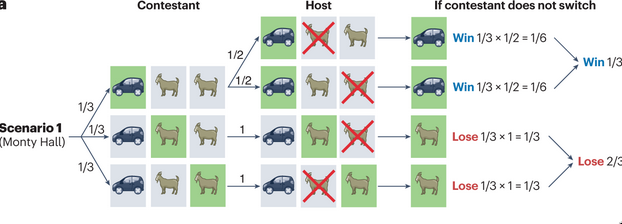
\includegraphics[width=0.8\textwidth]{assets/monty_hall_decision_tree.png}
  \caption{Monty Hall Decision Tree}
  \label{fig:monty_hall_decision_tree}
\end{figure}
When you select a goat, the host has to open the other goat box, restricting the choices (and thus influencing the 
probability of the events)

\subsection{Coupon Collector Problem}
There are $n$ prizes distributed in cereal boxes randomly, independently, and uniformly. 
You want randomly open cereal boxes with replacement until you have seen every prize at least once. 
Let $T_n$ = number of boxes you needed to open until you've seen all prizes. 
What is  $E[T_n]$?

\begin{proof}
  In other words, $T_n = \{\text{ first time # new coupons = n}\}$. We know that the time to collect
  first new coupon $=1$. 

  TODO when I have time.

\end{proof}
\end{document}
